\begin{question}[type=exam]{10}
  考虑一家公司的生产决策,其生产成本由下图中的边际成本 $MC$、平均可变成本 $AVC$ 和平均总成本 $ATC$ 曲线表示。

\begin{itemize}
  \item 假设在\textbf{短期}内,完全竞争市场的价格由图中标注为 $P$ 的水平线表示。\\
  请在图上说明该公司在短期内将生产的数量。
  \item 现在说明如果企业可以进入或退出市场,在\textbf{长期}内该市场将发生什么变化。\\
  请结合图像解释你的答案。
\end{itemize}
 

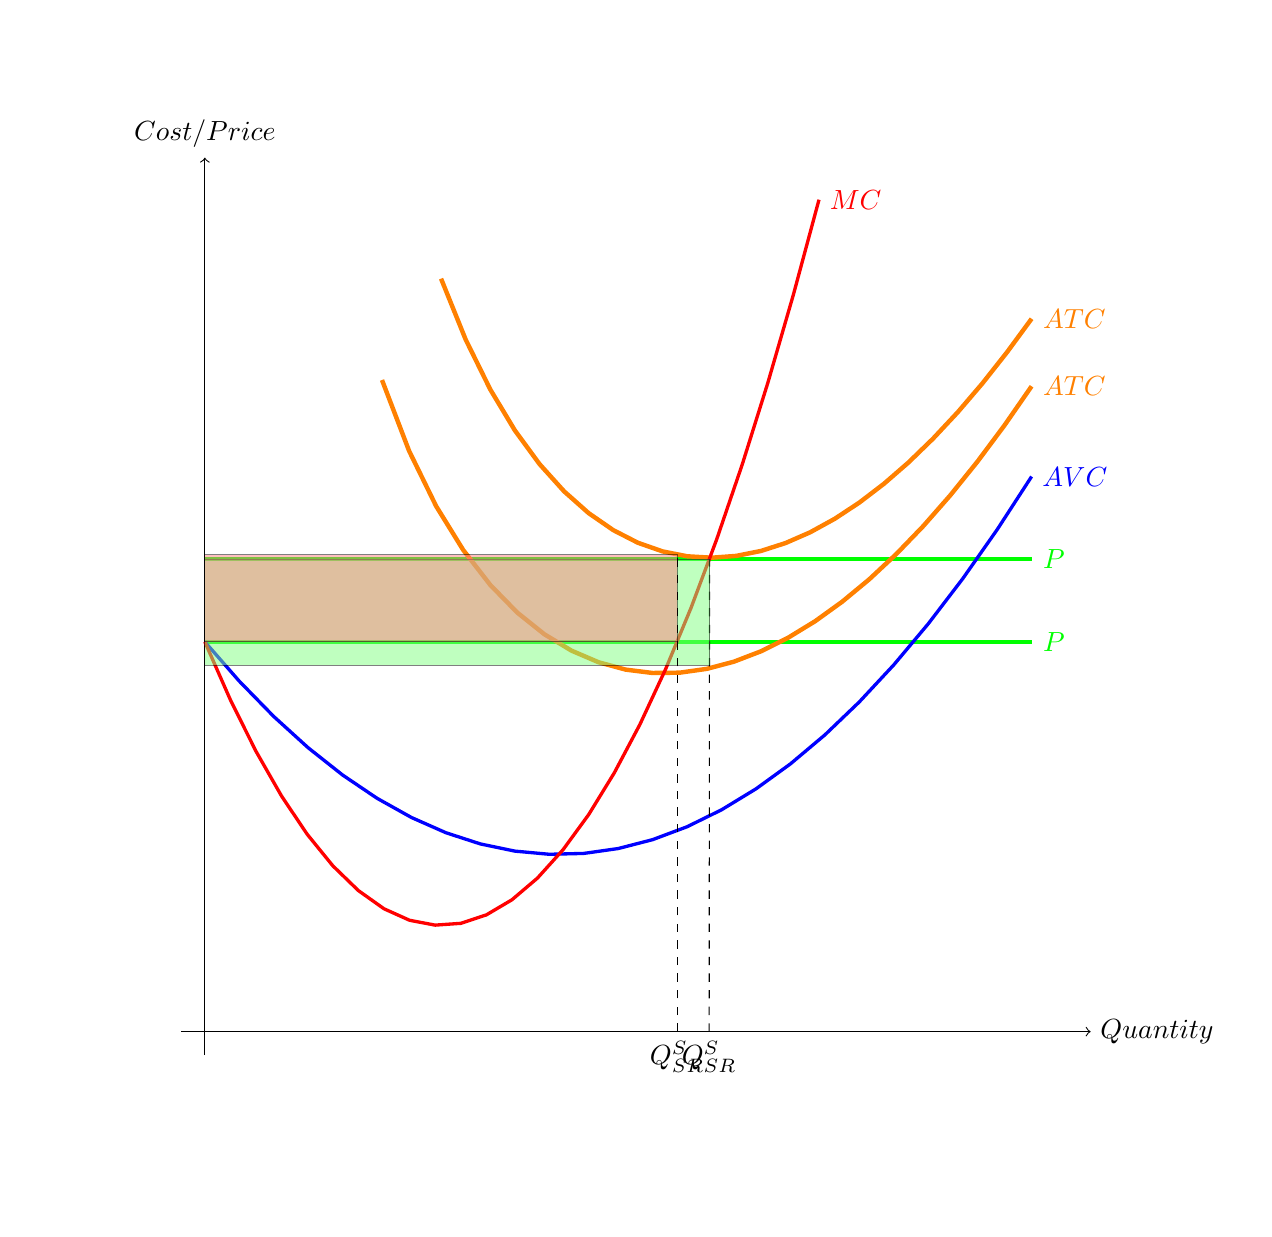
\begin{tikzpicture}[x=1.5cm, y=1.5cm]
  % Clip drawing region to y <= 12
  \clip (-1.5,-1.5) rectangle (8.8,8.5);

  % \draw[very thin,color=gray,style=dashed] (-0,-0) grid (7.1,6.5);

  \draw[->] (-0.2,0) -- (7.5,0) node[right] {$Quantity$};
  \draw[->] (0,-0.2) -- (0,7.4) node[above] {$Cost/Price$};

  % short run price
  \vary{
  \draw[ultra thick, color=green] (0,4)  -- (7,4) node[right] {$P$};
  }{
  \draw[ultra thick, color=green] (0,3.3)  -- (7,3.3) node[right] {$P$};
  }

  % cost curves
  \vary{
  \draw[ultra thick, color=orange, domain=1.5:7] plot (\x,{0.2*\x^2 - 1.2*\x + 3.3 + 5.35 / \x}) node[right] {$ATC$}; 
  }{
  \draw[ultra thick, color=orange, domain=2:7] plot (\x,{0.2*\x^2 - 1.2*\x + 3.3 + 9.35 / \x}) node[right] {$ATC$}; 
  }
  \draw[very thick, color=blue, domain=0:7] plot (\x,{0.2*\x^2 - 1.2*\x + 3.3}) node[right] {$AVC$}; 
  \draw[very thick, color=red, domain=0:5.2] plot (\x,{0.6*\x^2 - 2.4*\x + 3.3}) node[right] {$MC$}; 

  % solutions
  \PrintSolutionsTF{
    \vary{
      \draw[style=dashed] (4.27,0) node[below] {$Q^S_{SR}$} -- (4.273,4);
      \filldraw[fill=green!50, semitransparent] (0,3.1) rectangle (4.273,4);
    }{\draw[style=dashed] (4,0) node[below] {$Q^S_{SR}$} -- (4,4.0375);
      \filldraw[fill=red!50, semitransparent] (0,3.3) rectangle (4,4.0375);
    }
  }{}
\end{tikzpicture}


\PrintSolutionsTF{
  \fbox{\parbox{\linewidth}{
    
      
- 在短期中,利润最大化的供给量 $Q_{SR}^S$ 是 $P=MR$ 与 $MC$ 相交的位置。
      
- 
      \vary{
        在此短期情形中,企业的 $MR>ATC$,因此其利润为\textbf{正}。

        在图中,这对应于阴影矩形区域,其高度为 $P-ATC$,宽度为 $Q_{SR}^S$。

        在长期中,其他企业将\textbf{进入}市场,直到价格被\textbf{压低}至 $ATC$ 的最低点,此时所有企业获得零利润。
      }{
        在此短期情形中,企业的 $ATC>MR$,因此其利润为\textbf{负}。

        在图中,这对应于阴影矩形区域,其高度为 $ATC-P$,宽度为 $Q_{SR}^S$。

        在长期中,其他企业将\textbf{退出}市场,直到价格被\textbf{推高}至 $ATC$ 的最低点,此时所有企业获得零利润。
      }
    
    }
  }
  }{\vspace{5cm}}

\end{question}